\documentclass[10pt,conference,compsocconf]{IEEEtran}

\usepackage{hyperref}
\usepackage{amsmath}        % math
\usepackage{graphicx}   % For figure environment


\begin{document}
\title{Machine learning applied to the Higgs boson CERN dataset}

\author{
  Luc\'{i}a Montero Sanchis, Nuno Mota Gon\c{c}alves, Matteo Yann Feo,  \\
  \textit{Department of Computer Science, EPFL Lausanne, Switzerland}
}

\maketitle

\begin{abstract}
  This report presents the results of applying \textit{least squares} and \textit{logistic regression} to the Higgs boson dataset for classification purposes. These methods are analyzed and compared for different polynomial basis degrees of the input data. We also consider applying \textit{principal component analysis} to reduce the dimensionality of the feature space.
\end{abstract}

\section{Introduction}
	The aim of this project is to classify the data in CERN's dataset into two classes, for finding the Higgs boson. This task is carried out applying the machine learning methods learned during the course together with the improvements considered most appropriate, to overcome the challenges of the assignment. Some challenges include: handling the missing information in the dataset, properly dealing with a large number of features and samples and choosing the learning method that is the most suitable.

	The learning algorithms we focus on are \textit{least squares} and \textit{logistic regression}, being the latter the most adequate for classification. The possibility of including a regularization factor is considered in order to avoid over-fitting. We expand the features by including a polynomial basis up to a degree, to achieve a higher accuracy in the classification. We also use \textit{principal component analysis} (PCA) to obtain a smaller number of linearly uncorrelated variables.

	%We start by presenting the models and methods used in section \ref{sec:models-methods}. We then include the results obtained, and discuss them in section \ref{sec:discussion}.

\section{Models and methods}
	\label{sec:models-methods}
	\subsection{Initial data parsing} % (fold)
	\label{sub:initial_data_parsing}
  	The Higgs boson dataset contains $250,000$ observations and $30$ features. The variables take values in different ranges and some contain the value $-999.0$ for certain observations, which we consider to represent \emph{missing information}. %In some cases up to 29\% of the total observed data for a variable is missing.

  	Before applying a learning algorithm we standardize the features so that they are considered equally. To do so, we subtract the mean and divide by the standard deviation. For variables with missing information the mean and the standard deviation are computed only over the non-missing values. Afterwards the missing values are set to $0$ so that they do not modify the scale of the variable. When standardizing the test data we used the mean and the standard deviation of the train data to assure the same transformation on both datasets.%, although it should not make a big difference since the distribution of the training and test data is assumed to be the same.
	% subsection initial_data_parsing (end)

	\subsection{Polynomial basis} % (fold)
	\label{sub:polynomial_basis}
  	To improve the accuracy in the classification we increase the number of explanatory variables by building a polynomial basis. We expand the features including the powers of each of the original variables up to a certain chosen degree. Since the newly included variables may have a different standard deviation, we normalize them to assure that their standard deviation is $1$. We also include an offset term.
	% subsection polynomial_basis (end)

	\subsection{Principal Component Analysis (PCA)} % (fold)
	\label{sub:principal_component_analysis}
  	The total number of features increases considerably for polynomial basis with large degrees. In these cases we can reduce the dimensionality $d$ of the feature space using PCA.

  	As specified in \cite{smith02}, we first find the covariance matrix of the features. We then compute the eigenvalues and eigenvectors. The eigenvectors form a basis for the data and can be sorted in \emph{decreasing} order of eigenvalue. We can then select a subset of the first $L\leq d$ eigenvectors as basis vectors. This allows us to compare the results achieved for a polynomial basis of a \textit{larger} degree with the results achieved for a polynomial basis of a \textit{lower} degree - by reducing dimensionality when applying PCA.
	% subsection principal_component_analysis (end)

	\subsection{Least squares and Ridge regression} % (fold)
	\label{sub:least_squares_and_ridge_regression}
  	We start classifying with least squares. Since it is possible to have over-fitting, we considered the possibility of using ridge regression. However, the implemented ridge regression method penalizes the offset of the model, which might decrease the accuracy of the predictions.
	% subsection least_squares_and_ridge_regression (end)

	\subsection{Logistic regression and Regularized logistic regression} % (fold)
	\label{sub:logistic_regression_and_regularized_logistic_regression}
  	The focus then shifted towards \textit{logistic regression}, since it should be more suitable for classifying. For its implementation with \textit{stochastic gradient descent}, we set both a constant learning rate, $\lambda$, and an adaptive one, $\lambda^{(t)}$, as shown in \ref{eq:lr} (where $t$ represents the iteration).

  	\begin{equation}
    	\label{eq:lr}
      	\lambda^{(t)} = \eta \cdot t ^{- \kappa}
  	\end{equation}

  	Although using an adaptive learning rate increases the amount of hyper-parameters to adjust, the convergence improves.
  	Since there is a possibility of over-fitting - when considering a large degree for the polynomial basis - we contemplated  \textit{regularized logistic regression} instead, which adds a third hyper-parameter. The regularization implementation, in this case, does not penalize the offset term of the model, hence solving the problem mentioned previously.
	% subsection logistic_regression_and_regularized_logistic_regression (end)

	\subsection{Cross validation and hyper-parameter tuning} % (fold)
	\label{sub:cross_validation_and_hyperparameters_tuning}
  	We first consider a \textit{5-fold cross validation}. From the \emph{training} data, which represents $80\%$ of all the data, we then keep $80\%$ for training and assign $20\%$ for validation (i.e. for tuning the hyper-parameters). To compare the classification errors for each model, we define \emph{accuracy} as the ratio of correct predictions.	We choose the parameters for the adaptive learning rate $\lambda^{(t)}$ and the regularization factor $\gamma$ by using a random layout (random search).
	% subsection cross_validation_and_hyperparameters_tuning (end)

\section{Results}
\label{sec:results}
    We first predict the labels for the test data using \textit{least squares}, implemented using normal equations. Then, after building the polynomial basis for the training data with degrees from $2$ to $8$, we apply \textit{least squares} to it. Figure \ref{fig:LSprec} shows the accuracy obtained for the training, validation and test data for each maximum degree.

    \begin{figure}[htp]
      \centering
      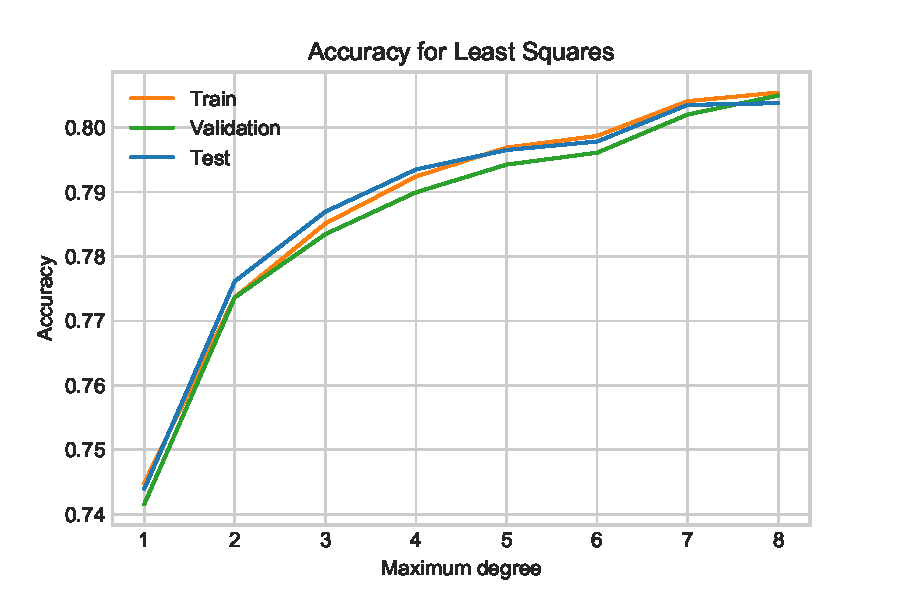
\includegraphics[width=.45\textwidth,trim={0 .3cm 0 .7cm},clip]{LSprec}
      \caption{Accuracy achieved using Least squares}
      \label{fig:LSprec}
    \end{figure}

    %\begin{figure}[htp]
      %\centering
      %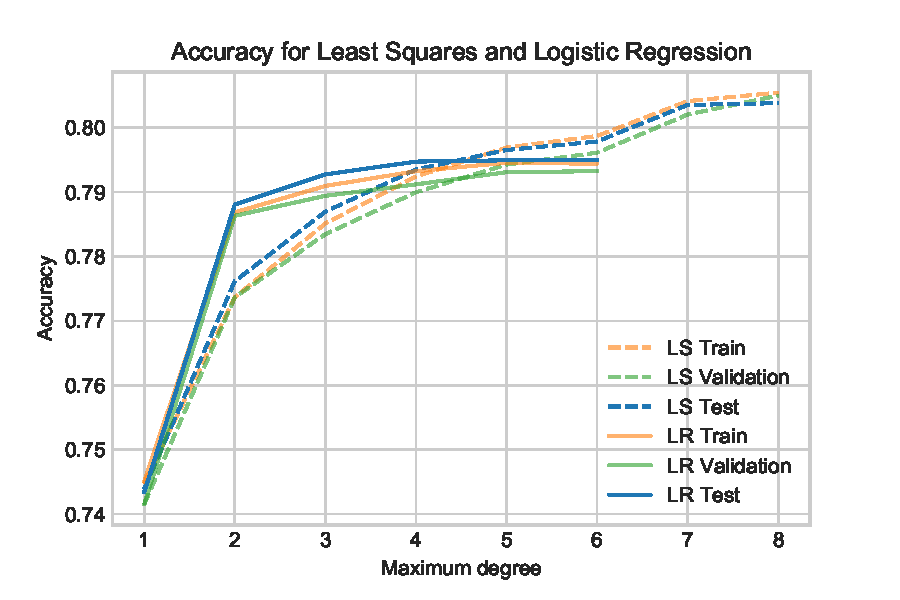
\includegraphics[width=.45\textwidth]{LSLRprec}
      %\caption{Accuracy achieved using Least squares and Logistic Regression}
      %\label{fig:LSLRprec}
    %\end{figure}

    We notice that the accuracy increases for larger maximum degrees but that it also stabilizes after a certain point. We also observe that there does not seem to be an over-fitting, since the difference in precision between the training and the validation-test predictions do not seem large.

    \begin{figure}[htp]
      \centering
      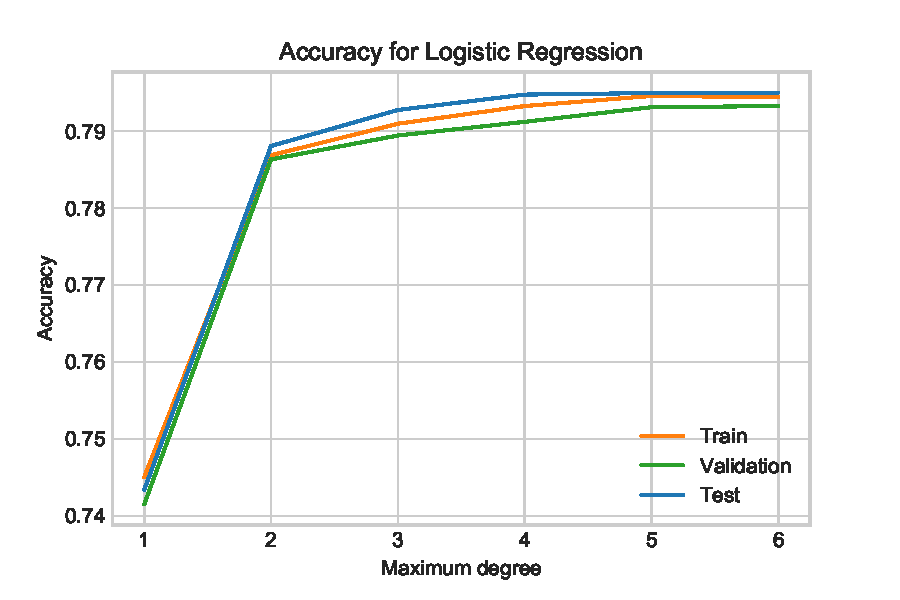
\includegraphics[width=.45\textwidth,trim={0 .3cm 0 .7cm},clip]{LRprec}
      \caption{Accuracy achieved using Logistic regression}
      \label{fig:LRprec}
    \end{figure}

    We then used \textit{logistic regression} with \textit{Stochastic Gradient Descent} (SGD), with $2,000$ batch size and $1,500$ iterations. As explained previously, we use an adaptive learning rate that is defined by two hyper-parameters. In this case, the values are $\eta = 10^{-2}$ and $\kappa = 0.8$. Figure \ref{fig:LRprec} shows the accuracy obtained for the training, validation and test data for each maximum degree using \textit{logistic regression}.
    In this case the accuracy, again, increases with the degree of the polynomial basis - and the model does not over-fit. Therefore, we do not include a regularization factor. As seen with \textit{least squares}, the increment in accuracy is smaller for larger degrees. Lastly, we compare the results for different \emph{maximum degrees}, keeping a constant number of features (first at $60$, then at $90$). The accuracy did not seem to depend on the degree, but instead on the number of features kept.

\section{Discussion}
\label{sec:discussion}
  In the results section we show that for polynomial basis of a larger degree there is a higher accuracy and more features to consider, when fitting the model. Moreover, it has also been shown that this difference in accuracy is larger for lower degree values. For instance, when using \textit{least squares} it is not clear whether or not considering a basis of degree $8$ is better than a basis of degree $7$. It is interesting as well to note that we did not find cases of over-fitting when using either \textit{least squares} or \textit{logistic regression}, probably due to the large size of the dataset.

  We also found that, although we expected the \textit{logistic regression} to perform better than \textit{least squares}, both algorithms achieve a similar accuracy for the same polynomial degree. In fact, for some degrees, \textit{least squares} outperforms \textit{logistic regression}. We speculate that this is caused by obtaining the analytical solution for \textit{least squares} versus estimating it for \textit{logistic regression} (by choosing a series of parameters, such as: learning rate, number of iterations and size of the batch for SGD).

  Lastly, we did find that as long as the number of features considered was the same, there were no changes in accuracy. Therefore, there were no improvements by using a large degree for the polynomial basis and applying PCA.

\section{Summary}
\label{sec:tips-writing}
  The difference in performance for \textit{least squares} and \textit{logistic regression} has not been large enough for us to take any final conclusions about which method is best for classification on this dataset. We have however seen that the accuracy is higher for either a higher degree of the polynomial basis or a higher feature space dimension. Increasing the degree and applying PCA, to reduce the number of features, does not improve the results for the cases considered.

\bibliographystyle{IEEEtran}
\bibliography{literature}

\end{document}
